\subsection{Architektury počítače}

\begin{definiceN}{Architektura počítača}
Architektura počítača popisuje \uv{všetko, čo by mal vedieť ten, ktorý programuje v assembleri / tvorí operačný systém}. Teda:
\begin{pitemize}
	\item z akých častí -- štruktúra počítača, usporadanie
	\item význam častí -- funkcia časti, ich vnútorná štruktúra
	\item ako spolu časti komunikujú -- riadenie komukácie
	\item ako sa jednotlivé časti ovládajú, aká je ich funkčnosť navonok
\end{pitemize}
\end{definiceN}

\begin{definiceN}{Víceúrovňová organizace počítače}
\begin{pitemize}
	\item Mikroprogramová úroveň (priamo technické vybavenie počítača)
	\item Strojový jazyk počítače (virtuálny stroj nad obvodovým riešením; vybavenie~-- popis architektúry a organizácie)
	\item Úroveň operačního systému (doplnenie predchádzajúcej úrovne o súbor makroinštrukcií a novú organizáciu pamäti)
	\item Úroveň assembleru (najnižšia úroveň ľudsky orientovaného jazyka)
	\item Úroveň vyšších programovacích jazyků (obecné alebo problémovo orientované; prvá nestrojovo orientovaná úroveň)
	\item Úroveň aplikačních programů
\end{pitemize}
\end{definiceN}


\begin{obecne}{Je teda potrebné definovať}
\begin{pitemize}
	\item Inštrukčný súbor (definícia prechodovej funkcie medzi stavmi počítača, formát inštrukcie, spôsob zápisu, možnosti adresovania operandov)
	\item Registrový model (rozlišovanie registrov procesoru: podľa voľby, pomocou určenia registru~-- explicitný/implicitný register; podľa funkcie registru~-- riadiaci~register/register~operandu)
	\item Definice specializovaných jednotek (jednotka na výpočet vo floatoch;\\fetch/decode/execute jednotky)
	\item Paralelismy (rozklad na úlohy, ktoré sa dajú spracovať súčasne~-- granularita (programy, podprogramy, inštrukcie...))
	\item Stupeň predikce (schopnosť pripraviť sa na očakávanú udalosť (načítanie inštrukcie, nastavenie prenosu dát)~-- explicitná predikcia, štatistika, heuristiky, adaptívna predikcia)

\bigskip
	\item Datové struktury a reprezentáciu dát (spôsob uloženia dát v počítači, mapovacie funkcie medzi reálnym svetom a vnútorným uložením, minimálna a maximálna veľkosť adresovateľné jednotky)
	\item Adresové konvencie (ako sa pristupuje k dátovým štruktúram~-- \emph{segment+offset} alebo \emph{lineárna adresácia}; veľkosť pamäti a jej šírika, \uv{povolené} miesta)

\bigskip
	\item Řízení (spolupráca procesoru a ostatných jednotiek, interakcia s okolím, prerušenia~-- vnútorne/vonkajšie)
	\item Vstupy a výstupy (metódy prenosu dát medzi procesorom a ostatnými jednotkami/počítačom a okolím; zahrňuje definície dátových štruktúr, identifikácia zdroja/cieľa, dátových ciest, protokoly, reakcie na chyby).
	\item Šíře datových cest
	\item Stupeň sdílení (na úrovni obvodov~-- zdieľanie obvodov procesoru a IO; na úrovni jednotiek~-- zdieľanie ALU viacerými procesormi)
\end{pitemize}
\end{obecne}

\subsubsection*{Základní dvě architektury počítačů}

\begin{obecne}{Von Neumannova}
  \begin{pitemize}
      \item Počítač se skládá z řídící jednotky, ALU, paměti a I/O jednotek
      \item Štruktúra počítača sa nemení typom úlohy (tj. počítač je programovaný obsahem paměti). %to tuetschek sorry neumim cist... ajs
      \item Program se nejprve zavede do paměti, z ní se postupně popořadě vybírají instrukce (a následující krok závisí na předchozím), pořadí lze změnit instrukcemi skoku. 
      \item Do jedné paměti, dělené na buňky stejné velikosti, se ukládají i zpracovávaná data. Data jsou reprezentovaná binárně. 
      \item V každém okamžiku je vykonávána jen jedna činnost. Je to architektura SISD (viz Flynnova taxonomie).
  \end{pitemize}

  Je pevně daná instrukční sada. Strojová instrukce obsahuje operační znak, který určuje druh operace, počet parametrů atd., a operandovú část~-- umístnění jednotlivých operandů. Vykonat jednu instrukci znamená:
  \begin{pitemize}
	  \item (fetch) načítať inštrukciu z pamäti do procesoru
	  \item (decode) zistiť o akú inštrukciu ide
	  \item (load) pripraviť zdrojové operandy
	  \item (execute) vykonať operáciu
	  \item (store) uloziť cieľové operandy
  \end{pitemize}

  Při vykonávání programu jsou potřebné různé registry~-- nejdůležitější jsou: PC (Program Counter, obsahuje adresu následující instrukce), IR (Instruction Register, adresa právě vykonávané instrukce), SP (Stack Pointer, ukazatel na vrchol zásobníku), MAR (memory access register~-- adresa do operační paměti), MBR (memory buffer register, dáta čítána/zapisována do paměti).

  Struktura jednoprocesorového počítače podle Von Neumanna:
  \begin{center}
    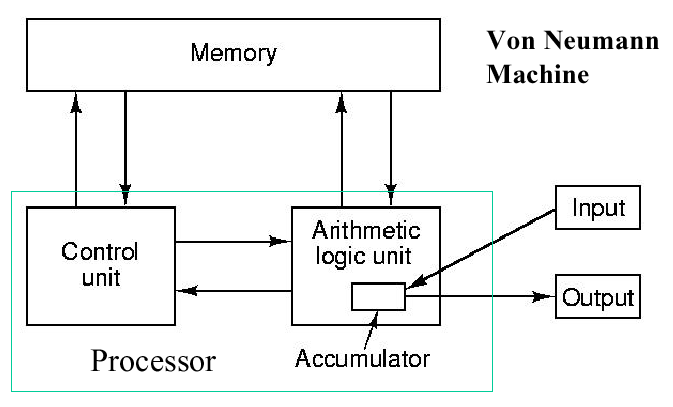
\includegraphics[width=8cm]{informatika/operacne_systemy_a_hw/obrazky/VonNeumann.png}
  \end{center}
\end{obecne}

\begin{obecne}{Harvardská}
Vytvořena až po Von Neumannově, liší se hlavně tím, že program se ukládá do jiné paměti než data (tzn. jsou 2 \uv{druhy paměti}~-- instrukcí a dat). Příklady jsou DSP procesory a mikrokontrolery (např. AVR od Atmelu, a PIC~-- mají paměť na program a data a RISC instrukční sadu; výhoda oddělených pamětí je, že můžou mít různou bitovou hloubku~-- 8 bitové data, ale 12-, 14- či 16- bitové instrukce (např. ARM musí občas použít více než jednou instrukci na zpracování obsahu plné velikosti)).

Oproti Von Neumannově nehrozí nebezpečí přepsání programu sebou samým, ale kvůli většímu počtu paměťových sběrnic je náročnější na výrobu. Paměť navíc nelze dělit podle potřeby (rozdělení je už dané).
\end{obecne}
